%\RequirePackage{fix-cm}
\documentclass[12pt, titlepage]{article}
\usepackage[title, titletoc]{appendix}
\usepackage{amssymb,amsmath}
\usepackage[backend=bibtex, style=nature, citestyle=nature, maxbibnames=2, isbn=false, date=year]{biblatex}
\usepackage{blindtext}
\usepackage{microtype}
%\usepackage{lettrine}
\usepackage{tikz}
\usetikzlibrary{matrix,arrows,positioning}
\usepackage{graphicx}

\frenchspacing

\addbibresource{Bibz.bib}

\begin{document}

\title{\textbf{\LARGE{Cooperativity in Dimerizing Systems}} \\[0.5em] \normalsize{Comparison of Epidermal Growth Factor an Estrogen Receptors}}
\author{Michael C. Fitzgerald}
\date{May 2016}
\maketitle

\begin{abstract}
%\lettrine{B}{y eight o'clock everything was ready}
By eight o'clock everything was ready, and we were on the other side of
the river.  We jumped into the stage, the driver cracked his whip, and we
bowled away and left ``the States" behind us.  It was a superb summer
morning, and all the landscape was brilliant with sunshine.  There was a
freshness and breeziness, too, and an exhilarating sense of emancipation
from all sorts of cares and responsibilities, that almost made us feel
that the years we had spent in the close, hot city, toiling and slaving,
had been wasted and thrown away.  We were spinning along through Kansas,
and in the course of an hour and a half we were fairly abroad on the
great Plains.  Just here the land was rolling--a grand sweep of regular
elevations and depressions as far as the eye could reach--like the
stately heave and swell of the ocean's bosom after a storm.  And
everywhere were cornfields, accenting with squares of deeper green, this
limitless expanse of grassy land.  But presently this sea upon dry ground
was to lose its ``rolling" character and stretch away for seven hundred
miles as level as a floor!
\end{abstract}
Tedte
\pagestyle{empty} %get rid of header/footer for toc page
\tableofcontents %put toc in
\clearpage %start new page
\pagestyle{plain} % put headers/footers back on
\setcounter{page}{1} %reset the page counter



\section{Introduction}
\blindmathtrue
\blindtext[2]
\begin{figure}
\centering
\includegraphics{grph4.pdf}
\caption{this is a nooj mode. Alkj fa lkj sdflkj dlkj;lkj akj fj kjkje alkjd flkjd lkjalksdf lkjdljadn lkc alkdlakjd nlja;lkj ff f fffff fookf l}
\end{figure}



\section{Models}
\blindtext[5]
\\ The lazy brown dog jumped over the office chairs fulfilling the prophecy.\supercite{notides_positive_1981, brandt_cooperativity_1997}

\begin{figure}%[h]
\centering
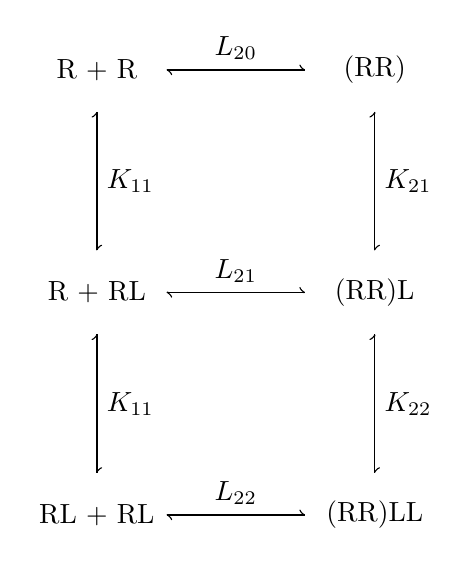
\begin{tikzpicture}
\tikzstyle{node}=[minimum height=3em, minimum width=5em, node distance = 5em]
\node[node](A) at (0,0)  {R + R};
\node[node](B) [below = of A] {R + RL};
\node[node](C) [below = of B]  {RL + RL};
\node[node](D) [right = of A] {(RR)};
\node[node](E) [below = of D] {(RR)L};
\node[node](F) [below = of E]  {(RR)LL};
\draw[-left to, line width=0.5pt] (A) -- node[right]{$K_{11}$} (B);
\draw[-left to, line width=0.5pt] (B) -- (A);
\draw[-left to, line width=0.5pt] (B) -- node[right]{$K_{11}$} (C);
\draw[-left to, line width=0.5pt] (C) -- (B);
\draw[-left to, line width=0.5pt] (A) -- node[above]{$L_{20}$} (D);
\draw[-left to, line width=0.5pt] (D) -- (A);
\draw[-left to, line width=0.5pt] (B) -- node[above]{$L_{21}$} (E);
\draw[-left to, line width=0.5pt] (E) -- (B);
\draw[-left to, line width=0.5pt] (C) -- node[above]{$L_{22}$} (F);
\draw[-left to, line width=0.5pt] (F) -- (C);
\draw[-left to, line width=0.5pt] (D) -- node[right]{$K_{21}$} (E);
\draw[-left to, line width=0.5pt] (E) -- (D);
\draw[-left to, line width=0.5pt] (E) -- node[right]{$K_{22}$} (F);
\draw[-left to, line width=0.5pt] (F) -- (E);
\end{tikzpicture}
\caption{this is a nugget model proposed by Wyman and Gill \supercite{wyman_binding_1990}}
\end{figure}

\blindtext[5]

\clearpage
\begin{appendices}
\section{Prism Code}
\blindtext[5]
\section{R Code}
\blindtext[5]
\end{appendices}

\clearpage
\printbibliography

\end{document}